%\chapter{RESULTADOS PRELIMINARES (Pt.1)}
\chapter{EMPILHAMENTO POR SUPERFÍCIE DE REFLEXÃO COMUM (SRC)}
\label{cap3}

Sendo desenhado para refletores pouco inclinados e pequenas variações laterais de velocidade da subsuperfície, e
para pequenos afastamentos fonte receptor as correções de sobretempo nem sempre são acuradas quando estas condições
são severamente violadas. \cite{tygel}

Na aquisição moderna, os dados sísmicos organizados em famílias de ponto médio comum (PMC) representam apenas uma fração
dos dados adquiridos. Como consequência, as expressões de sobretempo que usam posições arbitrárias dos pares fonte receptor
ao longo de um ponto central fixo (que pode ser inclusive um PMC) são aptas a fornecer melhor uso dos dados disponíveis
e usufruir da grande redundância que é oferecida. \cite{tygel}

O empilhamento por superfície de reflexão comum provém uma seção de afastamento nulo simulada a partir de dados sísmicos
de reflexão de multicobertura. Enquanto os métodos de imageamento convencionais requerem um macromodelo de velocidades
acurado para levar a resultados apropriados, o empilhamento por superfície de reflexão comum (SRC) não depende de um
macromodelo de velocidades \cite{jager}. 

O operador do empilhaento SRC é baseado em três atributos de duas frentes de ondas elementares
relacionadas ao raio de incidência normal \cite{hubral}:
Para a aquisição 2D, o empilhamento SRC produz uma superfície de empilhamento dependendente de três parâmetros.
A superfície de empilhamento ótima precisa ser determinada para cada ponto da seção de afastamento nulo simulada.
Para uma dada reflexão primária, estes parâmetros são o ângulo de emergência $\beta_0$ do raio de afastamento nulo, bem como
os raios de curvatura das frentes de onda $R_N$ e $R_{NIP}$, associados com duas frentes de onda hipotéticas,
a onda normal (N) e a onda de ponto de incidência normal (NIP) \cite{jager}.

Para cada ponto central $X_0$ na seção de afastamento nulo simulada com o empilhamento SRC, temos que determinar a tripla de
parâmetros ótimos ($\beta_0$, $R_N$ e $R_{NIP}$), a tripla para o qual o operador do empilhamento SRC ajusta melhor
os eventos de reflexão no domínio dos dados \cite{jager}.

A decomposição do campo de onda total sobre um conjunto de traços em partes correspondentes a diferentes ondas
de corpo é um dos problemas fundamentais do processamento de dados sísmicos. 
Em ordem de implementar esse procedimento é necessário
ter uma fórmula local de correção do tempo para uma família de pares fonte receptor distribuídos em volta de volta
de um par central escolhido.\cite{gelpart1}
De um ponto de vista físico, é possível corrigir todos os traços empilhados antes do empilhamento de uma maneira
que todos os eventos alvo estarão em fase. Assim, a operação crucial no empilhamento é a correção de tempo.\cite{gelpart1}

O empilhamento SRC no domínio do tempo desempenha um importante papel em várias técnicas de imageamento que independem do
conhecimento a priori do macromodelo de velocidades
\cite{peterhubral}:
Este estende o empilhamento convencional
ao longo de curvas de tempo de trânsito de reflexão no domínio do ponto médio comum (PMC) para
o empilhamento a partir de superfícies de reflexão comum (SRC) no domínio do meio afastamento $h$ - PMC $m$ \cite{fomel1}.
A aproximação do tempo de trânsito do empilhamento SRC depende dos raios de curvatura das frentes de onda
hipotéticas N e NIP, $R_N$ e $R_{NIP}$, e da velocidade próxima a superfície $v_0$. Ou seja, não depende
do conhecimento prévio do conhecimento a priori do macromodelo de velocidades.

O empilhamento SRC pode
ser compreendido a partir de dois experimentos hipotéticos esquematizados na Figura \ref{fig:3.1} \cite{gelpart1}: 
No primeiro, uma frente de onda (chamada NIP) se propaga para cima a partir de uma fonte pontual, 
originada no ponto de
reflexão do raio de afastamento nulo sobre o refletor alvo, ponto R. 
No segundo experimento hipotético, uma frente de onda (chamada N) se propaga para cima, produzida por um refletor explosivo na
vizinhança do ponto de reflexão R.
Em resumo, estas frentes de onda são definidas da seguinte forma \cite{tygel}: 

\begin{enumerate}
 \item A onda N inicia como uma frente de onda que coincide com o refletor, 
 propaga para cima com metade da velocidade do meio e chega ao ponto central $x_0$ no tempo $t_0$.

\item A onda NIP inicia no refletor alvo como uma fonte pontual no ponto de reflexão normal (R), propaga para
cima com metade da velocidade do meio e chega ao ponto central $x_0$ também no tempo $t_0$ .
\end{enumerate}


\begin{figure}[htb]
\caption{Representação esquemática das duas frentes de onda hipotéticas NIP (a) e N (b).}
\begin{center}
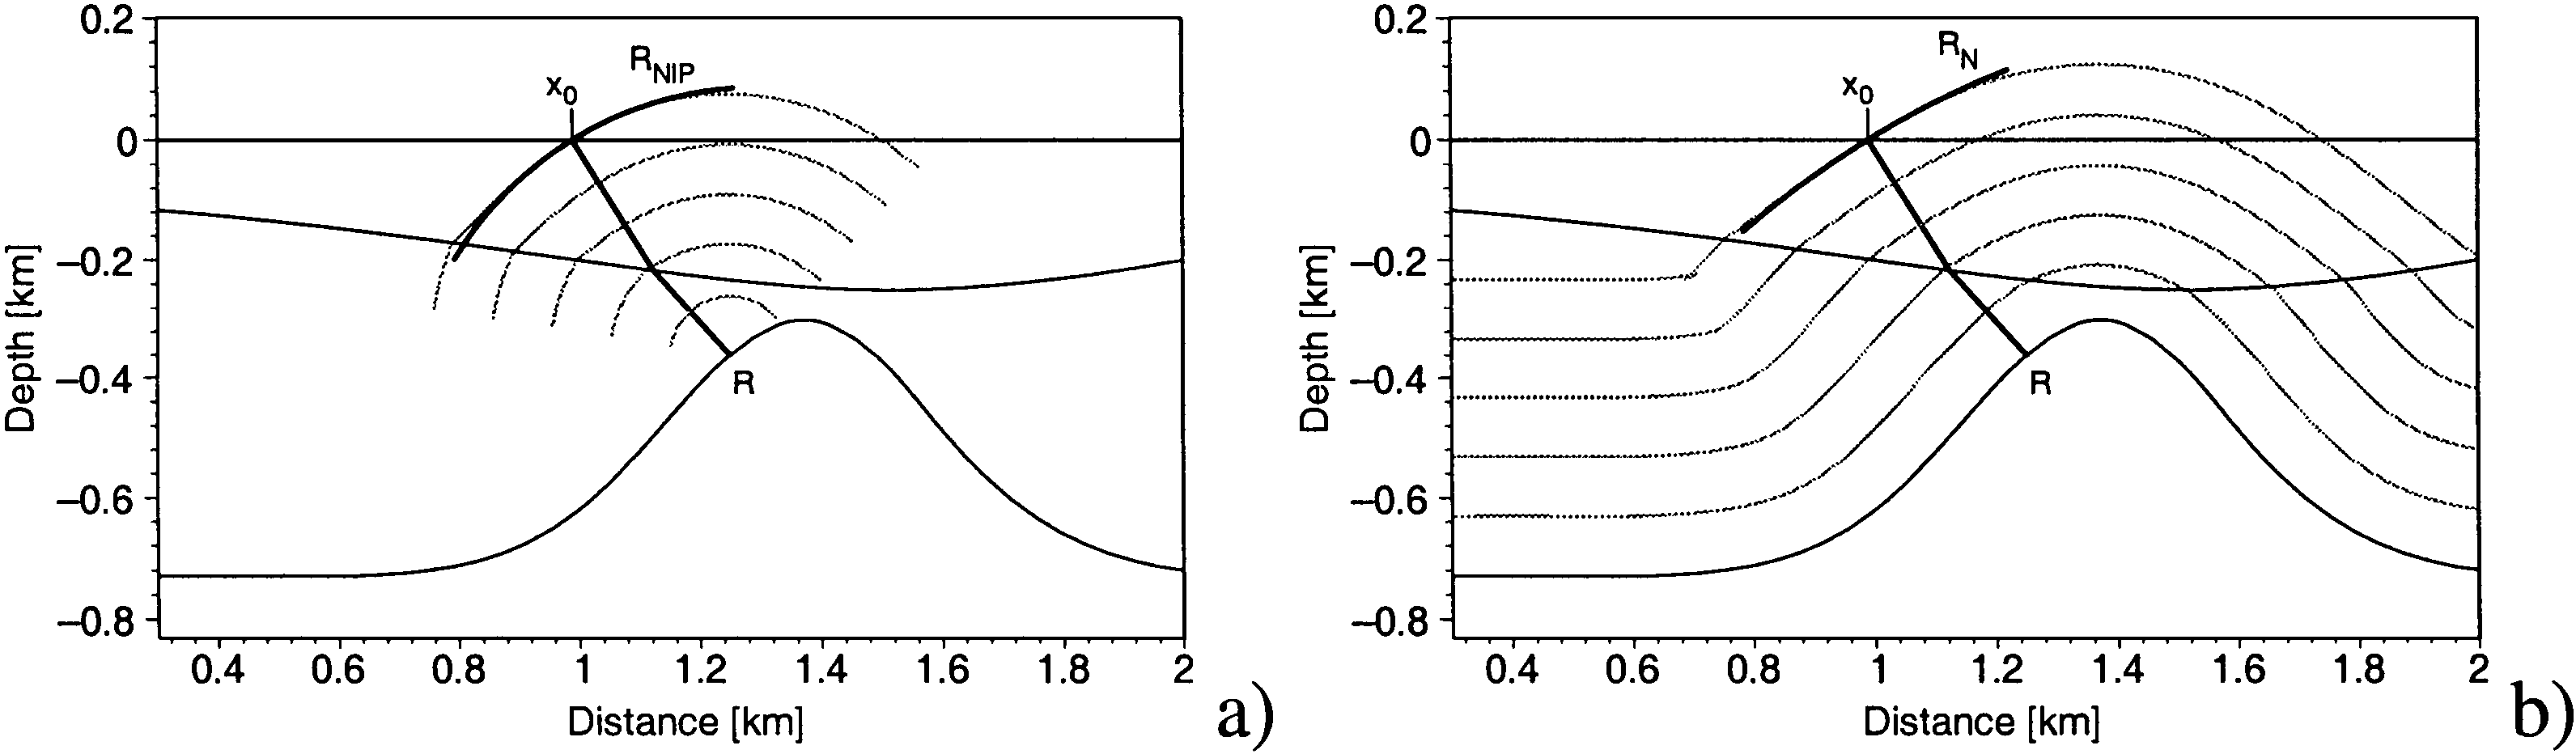
\includegraphics[scale=0.13]{images/crr.png}
\vspace{-0.3cm}
\end{center}
\begin{center}
 Fonte: Jager et al (2001).
\end{center}
\label{fig:3.1}
\end{figure}

O empilhamento CRS assume a seguinte forma:
Assumindo que os dados multicobertura são adquiridos em uma linha sísmica horizontal. Nesta linha, nós consideramos
uma reflexão primária de afastamento nulo fixa ou um raio central. Este raio é especificado a partir da coordenada $x_0$
que localiza o par fonte receptor correspondente e o ângulo de saída $\beta_0$. Reflexões primárias 
paraxiais são especificadas na vizinhança do raio central pelas coordenadas do ponto médio e do meio afastamento $(x_m,h)$.
O tempo de trânsito duplo do raio central é denotado por $t_0$ \cite{chirajc}.


\begin{equation}
\label{eq:3.1}
 S(t_0,m_0)=\int\int P(t(h,d=m-m_0;t_0)dhdm
\end{equation}


Onde a integral na Equação \ref{eq:3.1} ao redor de $m$ é realizada ao longo de uma vizinhança limitada de
um cmp central arbitrário $m_0$.
A superfície CRS $t(h,d)$ é uma função do
tempo de trânsito, em que $d=m_0-m$, é a distância entre o CMP central $m_0$ e um CMP na vizinhança $m$;
$h=x/2$ é o half-offset.
A superfície CRS $t(h,d)$ é uma aproximação do tempo de trânsito SRC o mais acurada possível. Várias
aproximações de tempo de trânsito SRC foram produzidas na literatura, como a aproximação hiperbólica do SRC
\cite{jager}, aproximação SRC quarta ordem \cite{germam}, aproximação não hiperbólica do SRC \cite{fomel1}
e aproximação do SRC Padé \cite{neves}, cada uma com as suas particularidades e graus de acurácia.

\section{APROXIMAÇÕES HIPERBÓLICA DO SRC}

A aproximação do SRC hiperbólico pode ser justificada como
uma expansão em série de Taylor, até segunda ordem, do quadrado do tempo de trânsito 
ao longo de um raio de referência \cite{fomel1}. A aproximação do CRS hiperbólico \cite{jager}:

\begin{equation}
\label{eq:3.2}
 \theta_{CRS}(h,d;t_0)=\sqrt{F(d)+b_2h^2}
\end{equation}


Onde:

\begin{equation}
\label{eq:3.3}
 F(d)=(t_0+a_1d)^2+a_2d^2
\end{equation}

\begin{equation}
\label{eq:3.4}
 a_1=\frac{2\sin(\beta_0)}{v_0}
\end{equation}

\begin{equation}
\label{eq:3.5}
 a_2=\frac{2\cos^2(\beta_0)t_0}{R_Nv_0}
\end{equation}

\begin{equation}
\label{eq:3.6}
 b_2=\frac{2\cos^2(\beta_0)t_0}{R_{NIP}v_0}
\end{equation}

\section{APROXIMAÇÃO NÃO HIPERBÓLICA DO SRC}

\cite{fomel1} propuseram a seguinte modificação de \ref{eq:3.67} com o intuito de melhorar a acurácia
para grandes offsets e separação entre os CMP's:

\begin{equation}
\label{eq:3.7}
 \Phi_{CRS}(h,d;t_0)=\sqrt{\frac{F(d)+ch^2+\sqrt{F(d-h)F(d+h)}}{2}}
\end{equation}


A Equação \ref{eq:3.7} é chamada equação do CRS não-hiperbólico. O parâmetros 
$a_1$, $a_2$ e $b_2$
do CRS hiperbólico são utilizados na definição
dos parâmetros do SRC não hiperbólico como:

\begin{equation}
\label{eq:3.8}
 c=2b_2+a_1^2-a_2
\end{equation}

\begin{equation}
\label{eq:3.9}
 F(d-h)=(t_0+a_1(d-h))^2+a_2(d-h)^2
\end{equation}

\begin{equation}
\label{eq:3.10}
 F(d+h)=(t_0+a_1(d+h))^2+a_2(d+h)^2
\end{equation}

\section{APROXIMAÇÕES DE QUARTA ORDEM DO SRC}

Com o intuito de aumentar a acurácia do método CRS para offsets longos e CMP's mais distantes do CMP central,
etendeu se o método CRS hiperbólico desenvolvendo 3 expansões 
em série de Taylor quarta ordem para a superfície CRS: 
$t(h,d)$ \textit{parabólica}, $t^2(h,d)$ \textit{hiperbólica} e $(t(h,d)-t_0+\frac{2}{v_0}R_{NIP})^2$
\textit{deslocada}. Chamado CRS quarta ordem, 
essas aproximações dependem dos mesmos parâmetros $v_0$, $R_N$, $R_{NIP}$ e $\beta_0$ do CRS hiperbólico,
porém acrescentam mais termos e qualidade à aproximação \cite{germam}.

\begin{multline}
\label{eq:3.11}
 t(h,d)=t_0+\frac{2\sin(\beta_0)}{v_0}d+\frac{\cos^2(\beta_0)}{v_0R_N}d^2+\frac{\cos^2(\beta_0)}{v_0R_{NIP}}h^2 \\
 -\frac{\sin(\beta_0)\cos^2(\beta_0)}{v_0R_N^2}d^3-\frac{\sin(\beta_0)\cos^2(\beta_0)}{v_0R_{NIP}^2R_N}(2R_{NIP}+R_N)dh^2 \\
 -\frac{\cos^2(\beta_0)}{2v_0R_{NIP}^3R_N^2}[R_{NIP}^2(8\cos^2(\beta_0)-6)+R_{NIP}R_N(5\cos^2(\beta_0)-4) \\
 -2R_N^2\sin^2(\beta_0)]h^2d^2-\frac{\cos^2(\beta_0)(5\cos^2(\beta_0)-4)}{4v_0R_N^3}d^4 \\
 +\frac{\cos^2(\beta_0)(4R_{NIP}\sin^2(\beta_0)-R_N\cos^2(\beta_0))}{4v_0R_{NIP}^3R_N}h^4 
\end{multline}

\begin{multline}
\label{eq:3.12}
 t^2(d,h)=t_0^2+\frac{4t_0\sin(\beta_0)}{v}d+2\frac{vt_0\cos^2(\beta_0)+2R_N\sin^2(\beta_0)}{v^2R_N}d^2+\frac{2t_0\cos^2(\beta_0)}{vR_{NIP}}h^2 \\
+\frac{2\sin(\beta_0)\cos^2(\beta_0)(2R_N-vt_0)}{v^2R_N^2}d^3 \\
+\frac{2\sin(\beta_0)\cos^2(\beta_0)(2R_{NIP}R_N-2vt_0R_{NIP}-vt_0R_N}{v^2R_{NIP}^2R_N})dh^2 \\
+\frac{\cos^2(\beta_0)}{v^2R_{NIP}^3R_N^2}[vt_0R_{NIP}^2(6-8\cos^2(\beta_0))+vt_0R_{NIP}R_N(4-5\cos^2(\beta_0)) \\
+2vt_0R_N^2\sin^2(\beta_0)-4R{NIP}R_N^2\sin^2(\beta_0)+R_{NIP}^2R_N(10\cos^2(\beta_0)-8)]d^2h^2 \\ 
+\frac{\cos^2(\beta_0)(R_N(10\cos^2(\beta_0)-8)+vt_0(4-5\cos^2(\beta_0))}{2v^2R_N^3}d^4 \\
+\frac{\cos^2(\beta_0)(4vt_0R_{NIP}\sin^2(\beta_0)-vt_0R_N\cos^2(\beta_0)+2R_{NIP}R_N\cos^2(\beta_0)}{2v^2R_{NIP}^3R_N}h^4
\end{multline}

\begin{multline}
\label{eq:3.13}
(t(h,d)-t_0+\frac{2}{v}R_{NIP})^2=(\frac{2}{v}R_{NIP})^2+\frac{8R_{NIP}\sin(\beta_0)}{v^2}d+4\frac{R_{NIP}\cos^2(\beta_0)+R_N\sin^2(\beta_0)}{v^2R_N}d^2 \\
+\frac{4\cos^2(\beta_0)}{v^2}h^2+\frac{4\sin(\beta_0)\cos^2(\beta_0)(R_N-R_{NIP}}{v^2R_N^2}d^3-\frac{8\sin(\beta_0)\cos^2(\beta_0)}{v^2R_N}dh^2 \\
+\frac{\cos^2(\beta_0)}{v^2R_N^3}[R_N(5\cos^2(\beta_0)-4)+R_{NIP}(4-5\cos^2(\beta_0))]d^4+\frac{4\cos^2(\beta_0)(3-4\cos^2(\beta_0))}{v^2R_N^2}d^2h^2 \\
+\frac{4\cos^2(\beta_0)\sin^2(\beta_0)}{v^2R_{NIP}R_N}h^4
\end{multline}


\section{APROXIMAÇÕES SRC PADÉ}

As aproximações do SRC quarta ordem dão origem a 6 aproximações de Padé do tempo de trânsito SRC, pois
cada uma das expansões do SRC quarta ordem pode ser expandida em duas aproximações de Padé, uma
no domínio do meio afastamento $h$ (oque equivale a manter $d$ constante e expandir em torno de $h$), e
no domínio da distância em relação ao PMC central $d$ (oque equivale a manter $h$ constante e 
realizar a aproximação de Padé tomando $h$ variável) \cite{neves}.

Para uma série de Taylor na forma; 
os coeficientes $\lambda$'s são constantes e $h$ é variável:

\begin{equation} %eq 7
\label{eq:3.14}
t^2(h) \approx \lambda_0+\lambda_1h^2+\lambda_2h^4+O(h^6)
\end{equation}

O aproximante de Padé [2/2] será dado por \cite{neves}:

\begin{equation} %eq 9
\label{eq:3.15}
 [2/2]=\zeta_1+\frac{h^2\zeta_2}{1+\zeta_3h^2}
\end{equation}

Onde:

\begin{equation}
\label{eq:3.16}
 \zeta_1=\lambda_0 
\end{equation}

\begin{equation}
\label{eq:3.17}
 \zeta_2=\lambda_1
\end{equation}

\begin{equation}
\label{eq:3.18}
 \zeta_3=\frac{-\lambda_2}{\lambda_1}
\end{equation}


Se a série de Taylor é expressa na forma da Equação \ref{eq:3.14}, o aproximante de Padé [2/2] desta série de Taylor 
será dado pela Equação \ref{eq:3.15}.

Para uma série de Taylor na forma; 
os coeficientes $\lambda$'s são constantes e $d$ é variável:

\begin{equation}
\label{eq:3.19}
 t^2(d) \approx \lambda_0+\lambda_1d+\lambda_2d^2+\lambda_3d^3+\lambda_4d^4
\end{equation}

O aproximante de Padé [2/2] será \cite{neves}:
\begin{equation}
\label{eq:3.20}
 [2/2]=\frac{p_0+p_1d+p_2d^2}{q_0+q_1d+q_2d^2}
\end{equation}

Onde:

\begin{equation}
\label{eq:3.21}
q_1=\frac{-\lambda_2-\lambda_3+\lambda_4\lambda_1}{\lambda_2^2-\lambda_3\lambda_1}
\end{equation}

\begin{equation}
\label{eq:3.22}
q_2=\frac{-\lambda_4-\lambda_3q_1}{\lambda_2}
\end{equation}

\begin{equation}
\label{eq:3.23}
 p_0=\lambda_0
\end{equation}

\begin{equation}
\label{eq:3.24}
 p_1=\lambda_1+\lambda_0q_1
\end{equation}

\begin{equation}
\label{eq:3.25}
p_2=\lambda_0q_2+\lambda_1q_1+\lambda_2
\end{equation}

O aproximante de Padé [2/2] da Equação \ref{eq:3.6} não possui uma forma compacta como a Equação \ref{eq:3.2}. 
No entanto, é
dado pela Equação \ref{eq:3.7} em função dos coeficientes $p$'s e `$q$'s nas Equações \ref{eq:3.8}-\ref{eq:3.12} 
que dependem
dos coeficientes da própria série de taylor aproximada (coeficientes $\lambda$'s).

\section{APROXIMAÇÃO PARA $t(h,d)$, EXPANSÃO EM h}
\label{sec:6.1}

A aproximação em série de Taylor quarta ordem da superfície CRS, desenvolvida por \cite{germam}, para $t(h,d)$:

\begin{multline}
\label{eq:6.13}
 t(h,d)=t_0+\frac{2\sin(\beta_0)}{v_0}d+\frac{\cos^2(\beta_0)}{v_0R_N}d^2+\frac{\cos^2(\beta_0)}{v_0R_{NIP}}h^2 \\
 -\frac{\sin(\beta_0)\cos^2(\beta_0)}{v_0R_N^2}d^3-\frac{\sin(\beta_0)\cos^2(\beta_0)}{v_0R_{NIP}^2R_N}(2R_{NIP}+R_N)dh^2 \\
 -\frac{\cos^2(\beta_0)}{2v_0R_{NIP}^3R_N^2}[R_{NIP}^2(8\cos^2(\beta_0)-6)+R_{NIP}R_N(5\cos^2(\beta_0)-4) \\
 -2R_N^2\sin^2(\beta_0)]h^2d^2-\frac{\cos^2(\beta_0)(5\cos^2(\beta_0)-4)}{4v_0R_N^3}d^4 \\
 +\frac{\cos^2(\beta_0)(4R_{NIP}\sin^2(\beta_0)-R_N\cos^2(\beta_0))}{4v_0R_{NIP}^3R_N}h^4 
\end{multline}

A variável onde será realizada a aproximação de Padé é $h=x/2$,
$d$ é mantido constante, e a aproximação de Padé [2/2] é realizada somente em $h$.
Definindo os coeficientes $\lambda$'s na forma:

\begin{equation}
\label{eq:6.14}
 \lambda_0=t_0+\frac{2\sin(\beta_0)}{v_0}d+\frac{\cos^2(\beta_0)}{v_0R_N}d^2-\frac{\sin(\beta_0)\cos^2(\beta_0)}{v_0R_N^2}d^3-\frac{\cos^2(\beta_0)(5\cos^2(\beta_0)-4)}{4v_0R_N^3}d^4
\end{equation}

\begin{multline}
\label{eq:6.15}
 \lambda_1=\frac{\cos^2(\beta_0)}{v_0R_{NIP}}-\frac{\sin(\beta_0)\cos^2(\beta_0)}{v_0R_{NIP}^2R_N}(2R_{NIP}+R_N)d \\
  -\frac{\cos^2(\beta_0)}{2v_0R_{NIP}^3R_N^2}[R_{NIP}^2(8\cos^2(\beta_0)-6)+R_{NIP}R_N(5\cos^2(\beta_0)-4)-2R_N^2\sin^2(\beta_0)]d^2
\end{multline}

\begin{equation}
\label{eq:6.16}
  \lambda_2=\frac{\cos^2(\beta_0)(4R_{NIP}\sin^2(\beta_0)-R_N\cos^2(\beta_0))}{4v_0R_{NIP}^3R_N}
\end{equation}

\begin{equation}
\label{eq:6.17}
  \frac{-\lambda_2}{\lambda_1}=-\frac{1}{2}\frac{Q_1}{Q_2}       
\end{equation}

Onde:

\begin{equation}
\label{eq:6.18}
Q_1=4R_{NIP}R_N\sin^2(\beta_0)-R_N^2\cos^2(\beta_0)
\end{equation}


\begin{multline}
\label{eq:6.19}
Q_2=2R_{NIP}^2R_N^2-2R_{NIP}R_N(2R_{NIP}+R_N)\sin(\beta_0)d \\
-[R_{NIP}^2(8\cos^2(\beta_0)-6)+R_{NIP}R_N(5\cos^2(\beta_0)-4)-2R_N^2\sin^2(\beta_0)]d^2
\end{multline}

Definindo os coeficientes $lambda$'s dessa forma, a Equação \ref{eq:3.13} se torna semelhante a
Equação \ref{eq:3.1}. Portanto,
o aproximante de Padé [2/2] da Equação \ref{eq:3.13} será dado também pela Equação \ref{eq:3.2}.

Substituimos os coeficientes $\lambda$'s definidos em \ref{eq:3.14}-\ref{eq:3.17} na definição dos coeficientes $\zeta$'s
nas Equações \ref{eq:3.3}-\ref{eq:3.5}:

\begin{equation}
\label{eq:6.20}
 \zeta_1=\lambda_0=t_0+\frac{2\sin(\beta_0)}{v_0}d+\frac{\cos^2(\beta_0)}{v_0R_N}d^2-\frac{\sin(\beta_0)\cos^2(\beta_0)}{v_0R_N^2}d^3-\frac{\cos^2(\beta_0)(5\cos^2(\beta_0)-4)}{4v_0R_N^3}d^4 
\end{equation}

\begin{multline}
\label{eq:6.21}
 \zeta_2=\lambda_1=\frac{\cos^2(\beta_0)}{v_0R_{NIP}}-\frac{\sin(\beta_0)\cos^2(\beta_0)}{v_0R_{NIP}^2R_N}(2R_{NIP}+R_N)d \\
  -\frac{\cos^2(\beta_0)}{2v_0R_{NIP}^3R_N^2}[R_{NIP}^2(8\cos^2(\beta_0)-6)+R_{NIP}R_N(5\cos^2(\beta_0)-4)-2R_N^2\sin^2(\beta_0)]d^2
\end{multline}

\begin{equation}
\label{eq:6.22}
 \zeta_3=\frac{-\lambda_2}{\lambda_1}=-\frac{1}{2}\frac{Q_1}{Q_2}  
\end{equation}


O aproximante de Padé [2/2] para $t(h,d)$ será dado pela Equação \ref{eq:3.1},
utilizando os coeficientes $\zeta$'s definidos nas Equações \ref{eq:3.20}-\ref{eq:3.22}, 
obtidos a partir dos coeficientes 
$lambda$'s definidos nas Equações \ref{eq:3.14}-\ref{eq:3.17}.

\section{APROXIMAÇÃO PARA $t^2(h,d)$, EXPANSÃO EM h}
\label{sec:6.2}

A aproximação em série de Taylor quarta ordem da superfície CRS, desenvolvida por \cite{germam}, para $t^2(h,d)$:


\begin{multline}
\label{eq:6.23}
 t^2(d,h)=t_0^2+\frac{4t_0\sin(\beta_0)}{v}d+2\frac{vt_0\cos^2(\beta_0)+2R_N\sin^2(\beta_0)}{v^2R_N}d^2+\frac{2t_0\cos^2(\beta_0)}{vR_{NIP}}h^2 \\
+\frac{2\sin(\beta_0)\cos^2(\beta_0)(2R_N-vt_0)}{v^2R_N^2}d^3 \\
+\frac{2\sin(\beta_0)\cos^2(\beta_0)(2R_{NIP}R_N-2vt_0R_{NIP}-vt_0R_N}{v^2R_{NIP}^2R_N})dh^2 \\
+\frac{\cos^2(\beta_0)}{v^2R_{NIP}^3R_N^2}[vt_0R_{NIP}^2(6-8\cos^2(\beta_0))+vt_0R_{NIP}R_N(4-5\cos^2(\beta_0)) \\
+2vt_0R_N^2\sin^2(\beta_0)-4R{NIP}R_N^2\sin^2(\beta_0)+R_{NIP}^2R_N(10\cos^2(\beta_0)-8)]d^2h^2 \\ 
+\frac{\cos^2(\beta_0)(R_N(10\cos^2(\beta_0)-8)+vt_0(4-5\cos^2(\beta_0))}{2v^2R_N^3}d^4 \\
+\frac{\cos^2(\beta_0)(4vt_0R_{NIP}\sin^2(\beta_0)-vt_0R_N\cos^2(\beta_0)+2R_{NIP}R_N\cos^2(\beta_0)}{2v^2R_{NIP}^3R_N}h^4
\end{multline}

A variável onde será realizada a aproximação é $h=x/2$,
$d$ é mantido constante, e a aproximação de Padé [2/2] é realizada somente em $h$.
Definindo os coeficientes $\lambda$'s na forma:

\begin{multline}
\label{eq:6.24}
 \lambda_0=t_0^2+\frac{4t_0\sin(\beta_0)}{V}d+2\frac{Vt_0\cos^2(\beta_0)+2R_N\sin^2(\beta_0)}{V^2R_N}d^2 \\
+\frac{2\sin(\beta_0)\cos^2(\beta_0)(2R_N-Vt_0)}{V^2R_N^2}d^3 \\
+\frac{\cos^2(\beta_0)(R_N(10\cos^2(\beta_0)-8)+Vt_0(4-5\cos^2(\beta_0))}{2V^2R_N^3}d^4 
 \end{multline}
 
\begin{multline}
\label{eq:6.25}
 \lambda_1=\frac{2t_0\cos^2(\beta_0)}{VR_{NIP}}+\frac{2\sin(\beta_0)\cos^2(\beta_0)(2R_{NIP}R_N-2Vt_0R_{NIP}-Vt_0R_N)}{V^2R_{NIP}^2R_N}d \\
+\frac{\cos^2(\beta_0)}{V^2R_{NIP}^3R_N^2}[Vt_0R_{NIP}^2(6-8\cos^2(\beta_0))+Vt_0R_{NIP}R_N(4-5\cos^2(\beta_0)) \\
+2Vt_0R_N^2\sin^2(\beta_0)-4R_{NIP}R_N^2\sin^2(\beta_0)+R_{NIP}^2R_N(10\cos^2(\beta_0)-8)]d^2
\end{multline}

\begin{equation}
\label{eq:6.26}
\lambda_2=\frac{\cos^2(\beta_0)(4Vt_0R_{NIP}\sin^2(\beta_0)-Vt_0R_N\cos^2(\beta_0)+2R_{NIP}R_N\cos^2(\beta_0)}{2V^2R_{NIP}^3R_N}
\end{equation}

\begin{equation}
\label{eq:6.27}
 [-\lambda_2/\lambda_1]=\frac{-R_NQ_3}{2}\frac{1}{(2Vt_0R_{NIP}^2R_N^2+2R_{NIP}R_NQ_1\sin(\beta_0)d+Q_2d^2)}
\end{equation}

Os coeficientes geométricos $Q$'s na Equação \ref{eq:3.27} são:

\begin{equation}
\label{eq:6.28}
 Q_1=2R_{NIP}R_N-2Vt_0R_{NIP}-Vt_0R_N
\end{equation}

\begin{multline}
\label{eq:6.29}
 Q_2=Vt_0R_{NIP}^2(6-8\cos^2(\beta_0))+Vt_0R_{NIP}R_N(4-5\cos^2(\beta_0)) \\
 +2Vt_0R_N^2\sin^2(\beta_0)-4R{NIP}R_N^2\sin^2(\beta_0)+R_{NIP}^2R_N(10\cos^2(\beta_0)-8)
\end{multline}

\begin{equation}
\label{eq:6.30}
 Q_3=4Vt_0R_{NIP}\sin^2(\beta_0)-Vt_0R_N\cos^2(\beta_0)+2R_{NIP}R_N\cos^2(\beta_0)
\end{equation}

Definindo os coeficientes $\lambda$'s dessa forma, a Equação \ref{eq:3.23} se torna semelhante a
Equação \ref{eq:3.1}. Portanto,
o aproximante de Padé [2/2] da Equação \ref{eq:3.23} será dado também por \ref{eq:3.2}.

Substituimos os coeficientes $\lambda$'s definidos nas Equações
\ref{eq:3.25}-\ref{eq:3.27} na definição dos coeficientes $\zeta$'s
em \ref{eq:3.3}-\ref{eq:3.5}:

\begin{multline}
\label{eq:6.31}
 \zeta_1=\lambda_0=t_0^2+\frac{4t_0\sin(\beta_0)}{V}d+2\frac{Vt_0\cos^2(\beta_0)+2R_N\sin^2(\beta_0)}{V^2R_N}d^2 \\
+\frac{2\sin(\beta_0)\cos^2(\beta_0)(2R_N-Vt_0)}{V^2R_N^2}d^3 \\
+\frac{\cos^2(\beta_0)(R_N(10\cos^2(\beta_0)-8)+Vt_0(4-5\cos^2(\beta_0))}{2V^2R_N^3}d^4 
\end{multline}

\begin{multline}
\label{eq:6.32}
 \zeta_2=\lambda_1=\frac{2t_0\cos^2(\beta_0)}{VR_{NIP}}+\frac{2\sin(\beta_0)\cos^2(\beta_0)(2R_{NIP}R_N-2Vt_0R_{NIP}-Vt_0R_N)}{V^2R_{NIP}^2R_N}d \\
+\frac{\cos^2(\beta_0)}{V^2R_{NIP}^3R_N^2}[Vt_0R_{NIP}^2(6-8\cos^2(\beta_0))+Vt_0R_{NIP}R_N(4-5\cos^2(\beta_0)) \\
+2Vt_0R_N^2\sin^2(\beta_0)-4R_{NIP}R_N^2\sin^2(\beta_0)+R_{NIP}^2R_N(10\cos^2(\beta_0)-8)]d^2
\end{multline}

\begin{equation}
\label{eq:6.33}
 \zeta_3=\frac{-\lambda_2}{\lambda_1}=\frac{-R_NQ_3}{2}\frac{1}{(2Vt_0R_{NIP}^2R_N^2+2R_{NIP}R_NQ_1\sin(\beta_0)d+Q_2d^2)} 
\end{equation}


O aproximante de Padé [2/2] para $t^2(h,d)$ será dado pela Equação \ref{eq:3.2},
utilizando os coeficientes $\zeta$'s definidos nas Equações \ref{eq:3.31}-\ref{eq:3.33}, 
obtidos a partir dos coeficientes 
$\lambda$'s definidos nas Equações \ref{eq:3.24}-\ref{eq:3.27}.


\section{APROXIMAÇÃO PARA $(t(d,h)-t_0+\frac{2}{v}R_{NIP})^2$, EXPANSÃO EM h}
\label{sec:6.3}
A aproximação em série de Taylor quarta ordem da superfície CRS, 
desenvolvida por \cite{germam}, para $(t(h,d)-t_0+\frac{2}{v}R_{NIP})^2$:

\begin{multline}
\label{eq:6.34}
(t(h,d)-t_0+\frac{2}{v}R_{NIP})^2=(\frac{2}{v}R_{NIP})^2+\frac{8R_{NIP}\sin(\beta_0)}{v^2}d+4\frac{R_{NIP}\cos^2(\beta_0)+R_N\sin^2(\beta_0)}{v^2R_N}d^2 \\
+\frac{4\cos^2(\beta_0)}{v^2}h^2+\frac{4\sin(\beta_0)\cos^2(\beta_0)(R_N-R_{NIP}}{v^2R_N^2}d^3-\frac{8\sin(\beta_0)\cos^2(\beta_0)}{v^2R_N}dh^2 \\
+\frac{\cos^2(\beta_0)}{v^2R_N^3}[R_N(5\cos^2(\beta_0)-4)+R_{NIP}(4-5\cos^2(\beta_0))]d^4+\frac{4\cos^2(\beta_0)(3-4\cos^2(\beta_0))}{v^2R_N^2}d^2h^2 \\
+\frac{4\cos^2(\beta_0)\sin^2(\beta_0)}{v^2R_{NIP}R_N}h^4
\end{multline}

A variável onde será realizada a aproximação é $h=x/2$,
$d$ é mantido constante, e a aproximação de Padé [2/2] é realizada somente em $h$.
Definindo os coeficientes $\lambda$'s na forma:

\begin{multline}
\label{eq:6.35}
 \lambda_0=(\frac{2}{v_0}R_{NIP})^2+\frac{8R_{NIP}\sin(\beta_0)}{v_0^2}d+4\frac{R_NIP\cos^2(\beta_0)+R_N\sin^2(\beta_0)}{v_0^2R_N}d^2 \\
 +\frac{4\sin(\beta_0)\cos^2(\beta_0)(R_N-R_{NIP}}{v_0^2R_N^2}d^3 \\
 +\frac{\cos^2(\beta_0)}{v_0^2R_N^3}[R_N(5\cos^2(\beta_0)-4)+R_{NIP}(4-5\cos^2(\beta_0))]d^4
 \end{multline}
 
\begin{equation}
\label{eq:6.36}
 \lambda_1=\frac{4\cos^2(\beta_0)}{v_0^2}-\frac{8\sin(\beta_0)\cos^2(\beta_0)}{v_0^2R_N}d+\frac{4\cos^2(\beta_0)(3-4\cos^2(\beta_0))}{v_0^2R_N^2}d^2
\end{equation}

\begin{equation}
\label{eq:6.37}
\lambda_2=\frac{4\cos^2(\beta_0)\sin^2(\beta_0)}{v_0^2R_{NIP}R_N}
\end{equation}

\begin{equation}
\label{eq:6.38}
 [-\lambda_2/\lambda_1]=-\frac{R_N\sin^2(\beta_0)}{R_{NIP}}\frac{1}{R_N^2-2R_N\sin(\beta_0)d+(3-4\cos^2(\beta_0))d^2}
\end{equation}

Definindo os coeficientes $\lambda$'s dessa forma, a Equação \ref{eq:3.34} se torna semelhante a
Equação \ref{eq:3.1}. Portanto,
o aproximante de Padé [2/2] da Equação \ref{eq:3.34} será dado também pela Equação \ref{eq:3.2}.

Substituimos os coeficientes $\lambda$'s definidos em \ref{eq:3.35}-\ref{eq:3.38} na definição dos coeficientes $\zeta$'s
nas Equações \ref{eq:3.3}-\ref{eq:3.5}:

\begin{multline}
\label{eq:6.39}
 \zeta_1=\lambda_0=(\frac{2}{v_0}R_{NIP})^2+\frac{8R_{NIP}\sin(\beta_0)}{v_0^2}d+4\frac{R_NIP\cos^2(\beta_0)+R_N\sin^2(\beta_0)}{v_0^2R_N}d^2 \\
 +\frac{4\sin(\beta_0)\cos^2(\beta_0)(R_N-R_{NIP}}{v_0^2R_N^2}d^3 \\
 +\frac{\cos^2(\beta_0)}{v_0^2R_N^3}[R_N(5\cos^2(\beta_0)-4)+R_{NIP}(4-5\cos^2(\beta_0))]d^4
\end{multline}

\begin{equation}
\label{eq:6.40}
 \zeta_2=\lambda_1=\frac{4\cos^2(\beta_0)}{v_0^2}-\frac{8\sin(\beta_0)\cos^2(\beta_0)}{v_0^2R_N}d+\frac{4\cos^2(\beta_0)(3-4\cos^2(\beta_0))}{v_0^2R_N^2}d^2
\end{equation}

\begin{equation}
\label{eq:6.41}
 \zeta_3=\frac{-\lambda_2}{\lambda_1}=-\frac{R_N\sin^2(\beta_0)}{R_{NIP}}\frac{1}{R_N^2-2R_N\sin(\beta_0)d+(3-4\cos^2(\beta_0))d^2} 
\end{equation}

O aproximante de Padé [2/2] para $(t(h,d)-t_0+\frac{2}{v}R_{NIP})^2$ será dado pela Equação \ref{eq:3.2},
utilizando os coeficientes $\zeta$'s definidos nas Equações \ref{eq:3.39}-\ref{eq:3.41}, a partir dos coeficientes 
$\lambda$'s definidos em \ref{eq:3.35}-\ref{eq:3.38}.

\section{APROXIMAÇÃO PARA $t(h,d)$, EXPANSÃO EM d}
\label{sec:6.4}
A variável onde será realizada a expansão é $d=m-mo$, 
para tanto $h$ é mantido constante e a aproximação de Padé {2/2] é realizada somente em $d$.
Se definimos os coeficientes $\lambda$'s na Equação \ref{eq:3.14} de modo que esta se torne semelhante 
a Equação \ref{eq:3.6},
o aproximante de Padé [2/2] da Equação \ref{eq:3.14} será dado pela Equação \ref{eq:3.7}.
Definindo os coeficientes $\lambda$'s da aproximação em série de Taylor quarta ordem da superfície CRS, 
desenvolvida por \cite{germam}, para $t(h,d)$ (Equação \ref{eq:3.14}):

%Definição dos coeficientes
\begin{equation}
\label{eq:6.42}
 \lambda_0=t_0+\frac{\cos^2(\beta_0)}{v_0R_{NIP}}h^2+\frac{\cos^2(\beta_0)(4R_{NIP}\sin^2(\beta_0)-R_N\cos^2(\beta_0))}{4v_0R_{NIP}^3R_N}h^4 
 \end{equation}
 
\begin{equation}
\label{eq:6.43}
 \lambda_1=\frac{2\sin(\beta_0)}{v_0}-\frac{\sin(\beta_0)\cos^2(\beta_0)}{v_0R_{NIP}^2R_N}(2R_{NIP}+R_N)h^2  
\end{equation}

\begin{multline}
\label{eq:6.44}
\lambda_2=\frac{\cos^2(\beta_0)}{v_0R_N}-\frac{\cos^2(\beta_0)}{2v_0R_{NIP}^3R_N^2}[R_{NIP}^2(8\cos^2(\beta_0)-6) \\
 +R_{NIP}R_N(5\cos^2(\beta_0)-4)-2R_N^2\sin^2(\beta_0)]h^2
\end{multline}

\begin{equation}
\label{eq:6.45}
\lambda_3=-\frac{\sin(\beta_0)\cos^2(\beta_0)}{v_0R_N^2}
\end{equation}

\begin{equation}
\label{eq:6.46}
\lambda_4=-\frac{\cos^2(\beta_0)(5\cos^2(\beta_0)-4)}{4v_0R_N^3}
\end{equation}

O aproximante de Padé será dado pela Equação \ref{eq:3.7}:
Os coeficientes dos polinômios $p(d)$ e $q(d)$ são obtidos por meio de \ref{eq:3.8}-\ref{eq:3.12},
utilizando os coeficientes $\lambda$'s definidos nas Equações \ref{eq:3.42}-\ref{eq:3.46}.

\section{APROXIMAÇÃO PARA $t^2(h,d)$, EXPANSÃO EM d}
\label{sec:6.5}
A variável onde será realizada a aproximação de Padé [2/2] é $d=m-mo$, 
para tanto $h$ é mantido constante e a aproximação de Padé é realizada somente em $d$.
Se definimos os coeficientes $\lambda$'s na Equação \ref{eq:3.23} de modo que esta se torne semelhante à \ref{eq:3.6},
o aproximante de Padé [2/2] da Equação \ref{eq:3.23} será dado por \ref{eq:3.7}.
Definindo os coeficientes $\lambda$'s da aproximação em série de Taylor quarta ordem da superfície CRS, 
desenvolvida por \cite{germam}, para $t^2(h,d)$ (\ref{eq:3.23}):

%Definição dos coeficientes
\begin{multline}
\label{eq:6.47}
 \lambda_0=t_0^2+\frac{2h^2t_0\cos^2(\beta_0)}{v_0R_{NIP}} \\
 +\frac{h^4\cos^2(\beta_0)(4v_0t_0R_{NIP}\sin^2(\beta_0)-v_0t_0R_N\cos^2(\beta_0)+2R_{NIP}R_N\cos^2(\beta_0))}{2v_0^2R_{NIP}^3R_N}
 \end{multline}
 
\begin{equation}
\label{eq:6.48}
 \lambda_1=\frac{4t_0\sin(\beta_0)}{v_0}+\frac{2\sin(\beta_0)\cos^2(\beta_0)(2R_{NIP}R_N-2v_0toR_{NIP}-v_0t_0R_N)h^2}{v_0^2R_{NIP}^2R_N}
\end{equation}

\begin{multline}
\label{eq:6.49}
\lambda_2=\frac{2(v_0t_0\cos^2(\beta_0)+2R_N\sin^2(\beta_0)}{v_0^2R_N} \\
+\frac{\cos^2(\beta_0)}{v_0^2R_{NIP}^3R_N^2}[v_0t_0R_{NIP}^2(6-8\cos^2(\beta_0))+v_0t_0R_{NIP}R_N(4-5\cos^2(\beta_0)) \\
+2v_0t_0R_N^2\sin^2(\beta_0)-4R_{NIP}R_N^2\sin^2(\beta_0)+R_{NIP}^2R_N(10\cos(\beta_0)-8)]h^2
\end{multline}

\begin{equation}
\label{eq:6.50}
\lambda_3=\frac{2\sin(\beta_0)\cos^2(\beta_0)(2R_N-v_0t_0)}{v_0^2R_N^2}
\end{equation}

\begin{equation}
\label{eq:6.51}
\lambda_4=\frac{\cos^2(\beta_0)(R_N(10\cos^2(\beta_0)-8)+v_0t_0(4-5\cos^2(\beta_0))}{2v_0^2R_N^3}
\end{equation}

O aproximante de Padé [2/2] será dado pela Equação \ref{eq:3.7}:
Os coeficientes dos polinômios $p(d)$ e $q(d)$ são obtidos por meio das Equações \ref{eq:3.8}-\ref{eq:3.12},
utilizando os coeficientes $\lambda$'s definidos nas Equações \ref{eq:3.47}-\ref{eq:3.51}.

\section{APROXIMAÇÃO PARA $(t(h,d)-t_0+\frac{2}{v_0}R_{NIP})^2$, EXPANSÃO EM d}
\label{sec:6.6}
A variável onde será realizada a aproximação de Padé [2/2] é $d=m-mo$, 
para tanto $h$ é mantido constante e a aproximação de Padé é realizada somente em $d$.
Se definimos os coeficientes $\lambda$'s na Equação \ref{eq:3.34} de modo que esta se torne semelhante 
a Equação \ref{eq:3.6},
o aproximante de Padé [2/2] da Equação \ref{eq:3.34} será dado por \ref{eq:3.7}.
Definindo os coeficientes $\lambda$'s da aproximação em série de Taylor quarta ordem da superfície CRS, 
desenvolvida por \cite{germam}, para $(t(d,h)-t_0+\frac{2}{v_0}R_{NIP})^2$ (Equação \ref{eq:5.34}):

%Definição dos coeficientes
\begin{equation}
\label{eq:6.52}
 \lambda_0=(\frac{2}{v_0}R_{NIP})^2+\frac{4\cos^2(\beta_0)}{v_0^2}h^2+\frac{4\cos^2(\beta_0)\sin^2(\beta_0)}{v_0^2R_{NIP}R_N}h^4
 \end{equation}
 
\begin{equation}
\label{eq:6.53}
 \lambda_1=\frac{8R_{NIP}\sin(\beta_0)}{v_0^2}-\frac{8\sin(\beta_0)\cos^2(\beta_0)}{v_0^2R_N}h^2 
\end{equation}

\begin{equation}
\label{eq:6.54}
\lambda_2=4\frac{R_NIP\cos^2(\beta_0)+R_N\sin^2(\beta_0)}{v_0^2R_N}+\frac{4\cos^2(\beta_0)(3-4\cos^2(\beta_0))}{v_0^2R_N^2}h^2
\end{equation}

\begin{equation}
\label{eq:6.55}
\lambda_3=\frac{4\sin(\beta_0)\cos^2(\beta_0)(R_N-R_{NIP}}{v_0^2R_N^2}
\end{equation}

\begin{equation}
\label{eq:6.56}
\lambda_4=\frac{\cos^2(\beta_0)}{v_0^2R_N^3}[R_N(5\cos^2(\beta_0)-4)+R_{NIP}(4-5\cos^2(\beta_0))]
\end{equation}


O aproximante de Padé [2/2] será dado pela Equação \ref{eq:3.7}:
Os coeficientes dos polinômios $p(d)$ e $q(d)$ são obtidos por meio das Equações \ref{eq:3.8}-\ref{eq:3.12},
utilizando os coeficientes $\lambda$'s definidos nas Equações \ref{eq:3.52}-\ref{eq:3.56}.



